\documentclass[../ro-fa-lab.tex]{subfiles}
\usepackage{hyperref}
\usepackage{graphicx}   % pachet pentru includerea imaginilor
\usepackage{xcolor}     % folosit de listings
\usepackage{listings}   % pentru blocuri de cod cu evidențiere
\lstset{
    language=C++,                   % limbajul (ii poți schimba la C, C, etc.)
    basicstyle=\ttfamily\small,     % font monospace, dimensiune mai mică
    keywordstyle=\color{blue},      % cuvinte cheie colorate
    commentstyle=\color{gray},      % comentarii colorate
    stringstyle=\color{red},        % șiruri de caractere colorate
    showstringspaces=false,         % nu afișează spații speciale în șiruri
    numbers=left,                   % numerotare linii pe stânga
    numberstyle=\tiny\color{gray},  % stil pentru numerele de linii
    frame=single,                   % chenar în jurul blocului de cod
    breaklines=true,                % rupe automat liniile lungi
    breakatwhitespace=true,         % rupe la spații dacă se poate
    tabsize=2                       % dimensiunea unui tab
}

\hypersetup{
    pdftitle={(RO) Erori},
    pdfauthor={},
    pdfsubject={},
    pdfkeywords={}
}

\begin{document}

\section{\textbf{Rezolvarea erorilor}}\label{errors}

\subsection{Profiler + VS Code error}\label{profiler-vscode-error}

În fișierul \texttt{Profiler.h} ai următoarele linii începând cu linia 11:

\begin{lstlisting}
// OS detection
#if defined(WIN32) || defined(_WIN32) || defined(__WIN32__) || defined(__NT__)
    #define PROFILER_WINDOWS
#elif __APPLE__
    #define PROFILER_OSX
#elif __linux__
    #define PROFILER_LINUX
#endif

#ifdef PROFILER_WINDOWS
    #include <Windows.h>
    #include <Shellapi.h>
#else
    #include <unistd.h>
#endif
\end{lstlisting}

Trebuie să le modifici în felul următor:

\begin{lstlisting}
// OS detection
#if defined(__MINGW32__) || defined(__CYGWIN__)
    #define PROFILER_VSCODE
#elif defined(WIN32) || defined(_WIN32) || defined(__WIN32__) || defined(__NT__)
    #define PROFILER_WINDOWS
#elif defined(__APPLE__)
    #define PROFILER_OSX
#elif defined(__linux__)
    #define PROFILER_LINUX
#endif

#if defined(PROFILER_WINDOWS) || defined(PROFILER_VSCODE)
    #include <Windows.h>
    #include <Shellapi.h>
#else
    #include <unistd.h>
#endif
\end{lstlisting}

Mai jos sunt capturile de ecran (în jur de 80\% din lățimea textului), încadrate ca figure:

\begin{figure}[htbp]
    \centering
    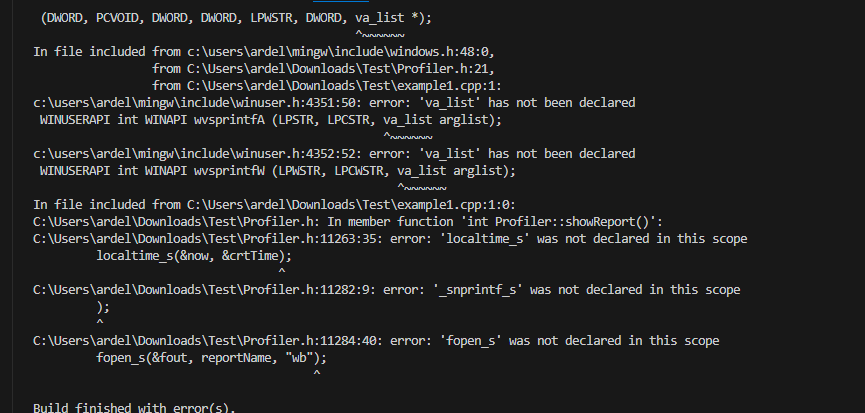
\includegraphics[width=0.8\textwidth]{./Resources/error_fix/image1.png}
    \caption{Eroarea inițială în VS Code Profiler}
    \label{fig:error1}
\end{figure}

\begin{figure}[htbp]
    \centering
    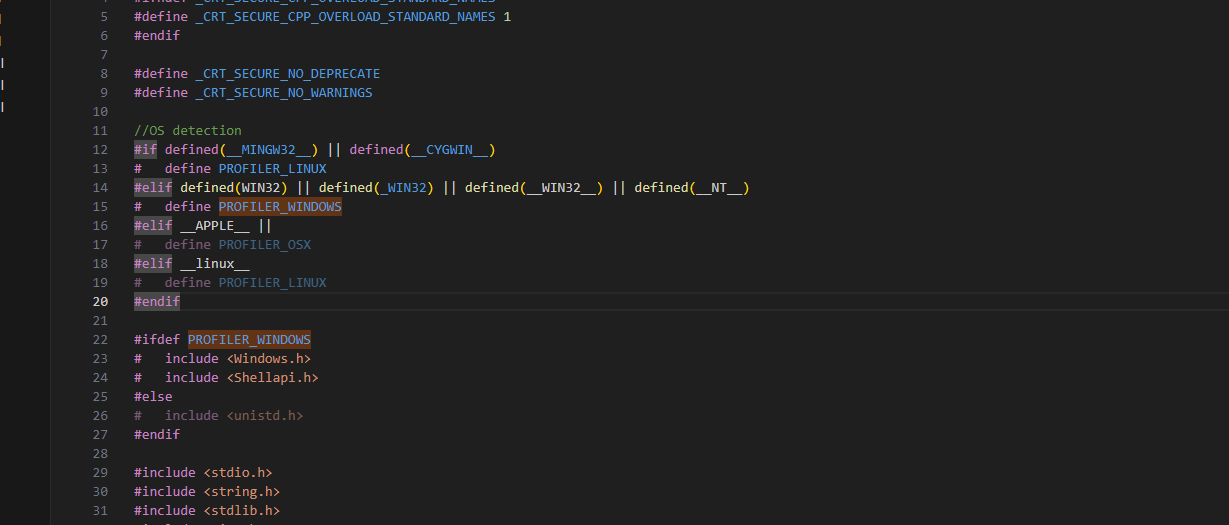
\includegraphics[width=0.8\textwidth]{./Resources/error_fix/image2.png}
    \caption{Captura de ecran originală (before fix)}
    \label{fig:error2}
\end{figure}

\begin{figure}[htbp]
    \centering
    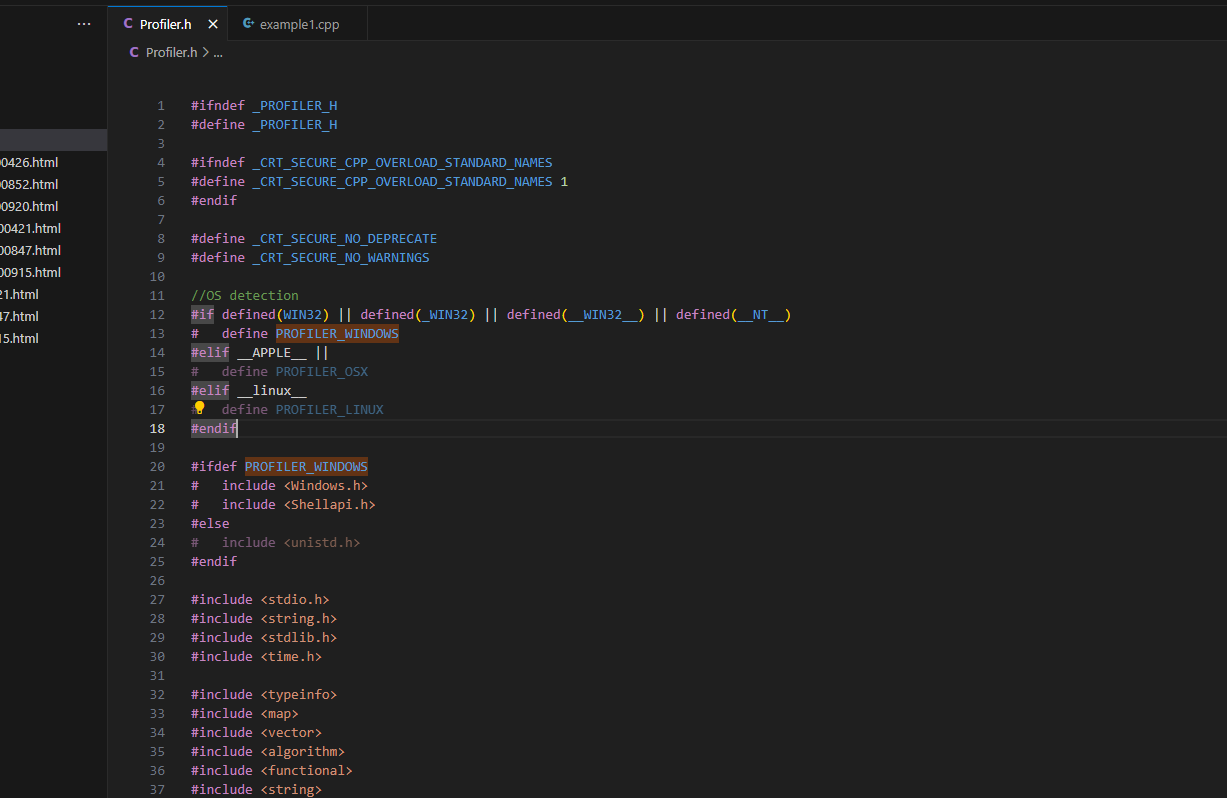
\includegraphics[width=0.8\textwidth]{./Resources/error_fix/image3.png}
    \caption{Captura de ecran după actualizare (after fix)}
    \label{fig:error3}
\end{figure}

\end{document}
